\chapter{Web Server - Workload Characterization}
L'obiettivo dell'homework è quello di realizzare un workload sintetico semplice e ripetibile, sulla base di un workload reale, attraverso le tecniche descritte nei capitoli precedenti. Successivamente esso deve essere applicato al sistema e, infine, si deve dimostrare che statisticamente si ottiene lo stesso risultato di un workload reale. L'esperimento può essere descritto in tre fasi:
\begin{enumerate}
	\item \textit{Simulazione di un workload reale}. In questa fase si simulano delle richieste random con carico prefissato al sistema. Si collezionano quindi i dati del client (lista delle richieste) di "alto livello" e i dati del server (memoria, utilizzo della CPU, ecc.) di "basso livello". Alla fine di questa fase bisogna analizzare i dati di alto livello per costruire un workload sintetico.
	\item \textit{Applicazione di un workload sintetico}. Dopo aver ricavato il workload sintetico al termine della fase precedente, esso deve essere applicato al sistema. Nuovamente quindi devono essere collezionati i dati di alto livello e basso livello.
	\item \textit{Validazione dei dati}. Prevede un'analisi approfondita dei dati di basso livello del workload reale e sintetico. Essi devono essere oppurtunamente caratterizzati per essere infine confrontati statisticamente. Per farlo si utilizzano dei test statistici meglio descritti successivamente.
\end{enumerate}
Le tre fasi possono essere rappresentate graficamente come nella successiva figura.

\begin{figure}[H]
	\centering
	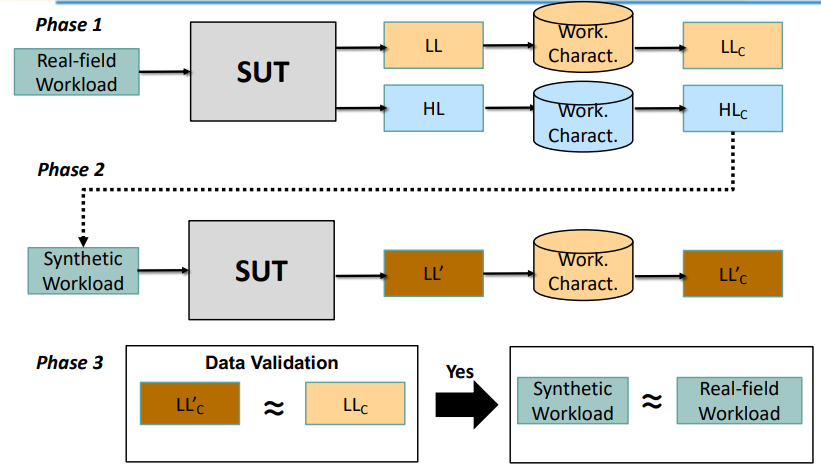
\includegraphics[width=0.6\textwidth]{img/hw3/Overview.png}
	\caption{\textit{Overview WL Characterization}}
\end{figure}

Per tutte le fasi il server occorre configurarlo allo stesso modo. In particolare si è utilizzato lo stesso Web Server descritto nel \textit{Capitolo 2} ma con una diminuzione di prestazioni solo a scopo didattico.

\section{Real-field Workload}
Per simulare quanto il più possibile un workload reale. Inoltre i dati di alto e basso livello devono essere presi contemporaneamente nel client e nel server.
\subsection{Server}
Il server contiene 10 file di diversa dimensione. I file sono stati scelti tutti dello stesso tipo (file di testo) solo per dimensionarli a piacimento. Nulla vieta però di utilizzare file di tipologie diverse (immagini, documenti, audio, etc.).
\\Essi sono stati dimensionati differenziando i file tra loro di 50 KB e partendo da un minimo di 50 KB.

\subsubsection{Parametri di basso livello}
Il web server è una macchina virtuale linux. Esistono dunque molti tool in grado di collezionare i parametri di caratteristici del sistema. In questo caso è stato utilizzato il tool \textbf{vmstat}. Esso offre inoltre la funzionalità di eseguire un campionamento dei parametri ad una frequenza e durata prefissata, tramite l'apposito comando eseguibile da terminale:
\begin{minted}[framesep = 1mm,
	fontsize = \footnotesize,
	breaklines,
	]{PYTHON}
	vmstat -n 1 400
\end{minted}
Il primo parametro "1" indica il periodo di campionamento in secondi, mentre il secondo parametro "400" indica la durata totale di esecuzione in secondi. L'output poi può essere semplicemente salvato in un file di testo.
\\Esso permette di monitorare parametri come:
\begin{itemize}
	\item \textit{free}, quantità di memoria libera.
	\item \textit{in}, numero di interruzioni al secondo
	\item \textit{us}, tempo trascorso dalla CPU nell'eseguire codice non-kernel
	\item \textit{sy}, tempo trascorso dalla CPU nell'eseguire codice kernel
	\item \textit{id}, tempo trascorso dalla CPU nello stato di idle
\end{itemize}
I quali poi devono essere opportunamente studiati.

\subsection{Client - JMeter}
La simulazione degli utenti che fanno accesso al server è stata possibile tramite il tool JMeter, già descritto nei capitoli precedenti. 
\\In particolare sono stati realizzati tre Thread Group ognuno composto da 10 Thread (l'equivalente di 10 utenti) con una durata di simulazione pari a 2 min ciascuno. Ogni gruppo contiene 10 richieste riferite alle 10 risorse disponibili nel web server. Esse vengono poi eseguite in modo casuale tramite un apposito controller. 
\begin{figure}[H]
	\centering
	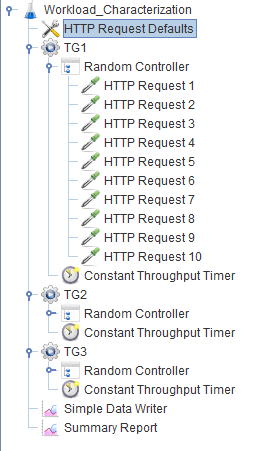
\includegraphics[width=0.4\textwidth]{img/hw3/jmeter_reale.png}
	\caption{\textit{Configurazione di JMeter per la simulazione di un workload reale}}
\end{figure}
Ogni gruppo inoltre ha un suo specifico carico. In questo caso si ha:
\begin{itemize}
	\item \textbf{TG1} : 400 richieste al minuto
	\item \textbf{TG2} : 550 richieste al minuto
	\item \textbf{TG3} : 700 richieste al minuto
\end{itemize}
Essi vengono poi eseguiti in sequenza e non in parallelo. Questo perché si possono creare possibili conflitti sulle risorse, dati dal fatto che ogni gruppo richiede le stesse risorse degli altri. 
\subsubsection{Parametri di alto livello}
I parametri di alto livello possono essere collezionati direttamente tramite il tool JMeter e salvati in formato \textit{.cvs}. Non sono necessari dunque programmi esterni. I parametri utili ai fini dell'analisi sono:
\begin{itemize}
	\item \textbf{Timestamp}, l'istante di tempo in cui viene effettuata la corrispettiva richiesta (in millisecondi)
	\item \textbf{elapse}, inteso come Response Time
	\item \textbf{label}, contiene l'informazione categorica della richiesta effettuata.
	\item \textbf{bytes}, numero di byte ricevuti tramite la relativa richiesta.
	\item \textbf{sentBytes}, numero di byte inviati per effettuare la richiesta.
	\item \textbf{latency}
	\item \textbf{connect}, tempo di connessione misurato per effettuare l'handshake TCP (in millisecondi).
\end{itemize}

\subsection{Workload Characterization}
Le misure vengono effettuate correttamente avviando prima \textit{vmstat} nel server e in seguito JMeter sul client in modo che i dati vengono salvati contemporaneamente nel lato client (alto livello) e nel lato server (basso livello). Al termine della simulazione quindi ci si ritrovano due file di dati.

\subsubsection{Parametri di alto livello}
I parametri di alto livello vanno incontro alla procedura di filtraggio, PCA e Clustering per ridurne la dimensionalità.
\\Essi appaiono nel seguente modo:
\begin{figure}[H]
	\centering
	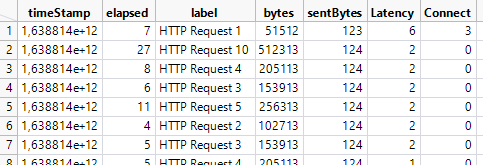
\includegraphics[width=0.8\textwidth]{img/hw3/alto_livello_esempio.png}
	\caption{\textit{Parametri di alto livello utili ai fini dell'analisi}}
\end{figure}
La fase di filtraggio non prevede nessuna azione di modifica del dataset.
\\Sul dataset originale quindi deve essere effettuata la PCA per cercare di ridurne la dimensionalità senza perdere troppa varianza. Bisogna soprattutto considerare che per questi parametri la fase di Clustering è molto importante poiché racchiude le informazioni principali per costruire il workload sintetico.
\\
\\
Tramite la PCA sono state scelte tutte le componenti principali, mantenendo una varianza del 100\%.
\begin{figure}[H]
	\centering
	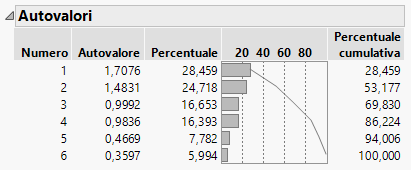
\includegraphics[width=0.6\textwidth]{img/hw3/autovalori.png}
	\caption{\textit{Analisi della varianza tramite autovalori}}
\end{figure}
\\
\\
Sulla base di queste può essere effettuato il clustering gerarchico.


\subsubsection{Parametri di basso livello}


\section{Synthetic Workload}
Collezionamento parametri basso livello wl sintetico
\\
Caratterizzazione parametri basso livello wl sintetico
\\
Random Selection su entrambi per identificare l'elemento rappresentativo di ogni cluster
\section{Data Validation}
Validazione del wl sintetico confrontando statisticamente i low level parameters ottenuti.